\documentclass[12pt]{article}

\usepackage{sbc-template}

\usepackage{graphicx,url}

%\usepackage[brazil]{babel}   
\usepackage[utf8]{inputenc}  

\usepackage{makecell}
     
\sloppy

\title{Modelos de Classificação de Sentimentos em \emph{Tweets} usando Programação Genética}

\author{Airton Bordin Junior\inst{1}}


\address{Instituto de Informática -- Universidade Federal de Goiás
  (UFG)\\
  Caixa Postal 131 -- 74690-900 -- Goiânia -- GO -- Brazil
}

\begin{document} 

\maketitle

\begin{abstract}
The increase in the number of Internet users in recent years has resulted in a growing content production by its users. Often, the WEB is used as a platform for debates, opinions, evaluations, etc. This fact, in line with the ease of obtaining the information, made the area of Sentiment Analysis, also called Opinion Mining, a growing interest on the part of reserachers.

One of the most used strategies in the process of Sentiment Analysis is the Lexical Dictionaries - a set of words and their polarities, generally defined as positive, negative or neutral. Although widely used, this approach has some challenges to overcome, such as identifying the domain of the text, for example - a word can have a completely different meaning depending on the context in which it is found.

[continue]
\end{abstract}

\begin{resumo} 
O aumento no número de usuários de Internet nos últimos anos teve como consequência uma crescentre produção de conteúdo por seus usuários. Frequentemente, a WEB é utilizada como plataforma para debates, opiniões, avaliações, etc. Esse fato, alinhado a facilidade de obtenção dessas informações, fez com que a área de Análise de Sentimentos, também chamada de Mineração de Opiniões, tivesse um interesse crescente por parte de pesquisadores. 

Uma das estratégias mais utilizadas no processo de Análise de Sentimentos é a utilização de Dicionários Léxicos  - conjunto de palavras e suas polaridades, geralmente definidas como positiva, negativa ou neutra. Apesar de amplamente utilizada, essa abordagem possui alguns desafios a serem superados, como a identificação do domínio do texto, por exemplo - uma palavra pode ter um significado completamente diferente, dependendo do contexto em que se encontra.

[continuar]
\end{resumo}

\section{Introdução}


\section{Análise de Sentimentos}
A Análise de Sentimentos, também chamada de Análise de Opiniões ou Mineração de Opiniões, é uma linha de pesquisa abrangente e que vem sendo tema de diversos trabalhos nos últimos anos. Como observado em \cite{liu2010multifaceted}, esse crescente interesse sobre o assunto ocorre principalmente devido ao aumento no número de usuários de Internet e o consequente crescimento da produção de conteúdo independente na rede, como opiniões, avaliações, entre outros. 

Essa área de estudo tem como principal desafio a Análise de Opiniões, descritas em linguagem natural, para a identificação da polaridade implícita ou explícita no texto. Essa polaridade é, na maior parte das vezes, identificada como uma escala de pontuação de sua característica positiva, negativa ou neutra.

Uma das principais técnicas para aumentar a acurácia a Análise de Sentimentos é a utilização de Dicionários de Dados. Esses dicionários contêm palavras previamente avaliadas por especialistas humanos, principalmente quanto à sua polaridade. Neste contexto, esse conjunto de palavras, juntamente com suas polaridades, é chamado de Dicionário Léxico ou Dicionário de Sentimentos. 

Porém, é evidente a limitação inerente à estratégia de utilização do Dicionário Léxico - a própria lista de palavras disponíveis. Esse fato muitas vezes limita a realização de uma análise mais profunda sobre determinado contexto. Nesse sentido, um dos principais desafios na área de Mineração de Opiniões é a criação e ampliação do Dicionário Léxico de forma automatizada, tema central do presente trabalho. Grande parte desses dicionários são construídos de forma manual, fato que caracteriza uma limitação óbvia para a maior parte dos contextos e domínios, como observado em \cite{duwairi2015detecting}. 

Existem, basicamente, 3 formas de criação e expansão de um Dicionário Léxico: manual -  processo realizado por especialistas humanos que analisam cada palavra, atribuindo uma Orientação Semântica para cada uma delas -  e duas formas (semi) automatizadas: baseada em Dicionário e baseada em Corpus. Frequentemente, essas técnicas são utilizadas em conjunto, principalmente a validação manual de Dicionários criados de forma automatizada. Criações de Dicionários utilizando somente abordagem manual, por sua característica limitante, são menos utilizadas e não serão abordadas de forma mais aprofundada no decorrer deste trabalho.

Consciente do problema de criação e expansão de Dicionários Léxicos para a Análise de Sentimentos, a ideia principal do presente trabalho é a [descrever aqui]

\section{Programação Genética}
Programação Genética é um campo da computação evolucionária que busca resolver problemas, de forma automatizada, sem demandar conhecimentos detalhados sobre a solução \cite{koza1992genetic}. De forma geral, podemos definir a Programação Genética como um método sistemático, não dependente de um domínio específico, usado para permitir que computadores criem programas para solução de problemas de forma automática, inciando com um conhecimento de alto nível sobre as regras gerais dos possíveis modelos.

Nesse contexto, programa significa um modelo capaz de, à partir de uma ou mais entradas, produzir uma saída para as mesmas. Embora possam ser representadas por diversos tipos de estruturas, a forma mais comum de representação é por meio de árvores, onde os nós internos representam funções e os nós folha representam terminais do problema. Um exemplo de um programa pode ser visto na figura \ref{treeProgram} \cite{Sannino2015}.

\begin{figure}[!htb]
	\centering
	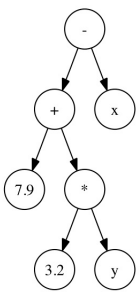
\includegraphics{programTree2}
	\caption{Programa representado a expressão (7.9 + (3.2 \* y) - x)}
	\label{treeProgram}
\end{figure}

Na Programação Genética, assim como em outros algoritmos baseados na evolução humana, são criadas populações onde cada indivíduo representa uma possível solução para o problema. A forma mais comum de inicialização da população é fazê-las de forma aleatória, evoluindo as mesmas no decorrer dos ciclos, chamados de gerações. Para cada geração, programas possivelmente melhores são criados, evoluindo os programas gerados. Assim como a natureza, a Programação Genética é um processo aleatório, e não garante o resultado ótimo. Porém, essa aleatoriedade faz com que, muitas vezes, as soluções fujam de problemas como soluções máximas locais, frequentemente enfrentado por métodos determiníticos gulosos \cite{mcphee2008field}.

\begin{figure}[!htb]
	\centering
	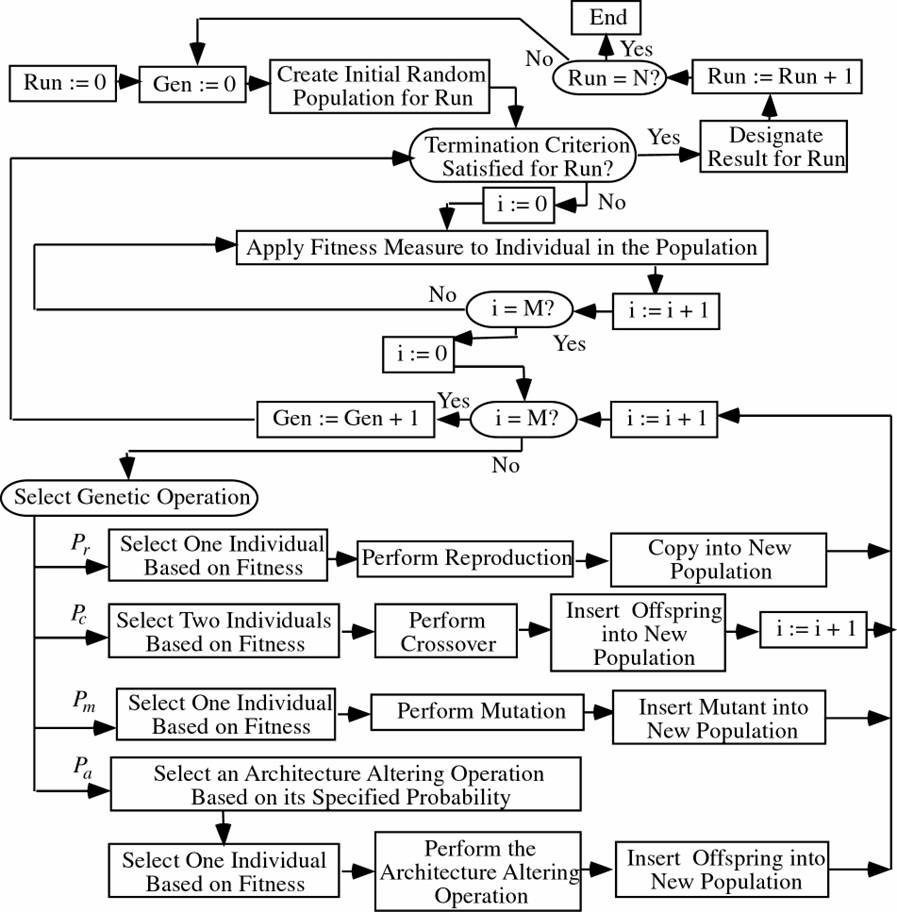
\includegraphics{GPFlowChart}
	\caption{Fluxograma da Programação Genética}
	\label{flowchart GP}
\end{figure}

Uma das características mais importantes da Programação Genética é a função de aptidão, ou função \emph{fitness}. Essa função busca representar, de forma quantitativa, a similaridade de cada indivíduo em relação ao resultado esperado. A escolha de uma boa função \emph{fitness} está intimamente ligada ao tipo do problema.

Os responsáveis pela evolução da população de indivíduos são os operadores genéticos. Para a Programação Genética, os principais operadores são a seleção, mutação e \emph{crossover}. Na seleção, um indivíduo é escolhido para fazer parte da próxima geração. A mutação modifica um nó da árvore, de forma a criar um indivíduo modificado em uma das partes escolhida aleatoriamente. O \emph{crossover} realiza o cruzamento entre dois indivíduos (pais), gerando duas novas possíveis soluções para o problema (filhos). Além desses principais operadores, existem outros como a edição, encapsulamento e a destruição \cite{patelli2011genetic}.

[Colocar mais informações aqui?]

O processo de criação e evolução de indivíduos e gerações pode ser visto em detalhes no fluxograma apresentado na figura \ref{flowchart GP}

\section{Trabalhos relacionados}

\label{sec:bibl}

A Análise de Sentimentos é uma linha de pesquisa multidisciplinar, podendo ser considerada uma subárea de Processamento de Linguagem Natural (PNL), como afirma \cite{liu2010multifaceted}. O autor, um dos principais nomes sobre o assunto, conceitualiza o problema e propõe uma forma estruturada de organização dos dados não estruturados, característica instínseca dos textos em linguagem natural, objeto de entrada da pesquisa. A definição de opinião como uma quíntupla (entidade, aspecto da entidade, sentimento, autor e tempo) é utilizada em grande parte dos trabalhos na área, caracterizando-se, portanto, como elemento fundamental nas pesquisas sobre o assunto. Visão geral sobre o tema e principais desafios e técnicas são vistos também em \cite{mohammad2016challenges}, \cite{ghaleb2016survey}, \cite{kdir16}, \cite{taboada2011lexicon}, \cite{bandhakavi2016lexicon}, \cite{Alessia}, entre outros trabalhos.

No contexto de prognóstico automatizado de Orientação Semântica de palavras, um dos primeiros trabalhos apresentados foi \cite{Hatzivassiloglou}, focando na previsão de polaridade de adjetivos.

Uma forma de prever a polaridade sentimental de palavras desconhecidas é levar em consideração aspectos sintáticos e semânticos do texto. \cite{Turney2002} apresenta uma abordagem de expansão léxica fazendo uso da técnica de \emph{Pointwise Mutual Infomation} (PMI), com o objetivo de calcular a co-ocorrência de palavras e, com isso, comparar a polaridade de novas palavras com outras já conhecidas. Nesse trabalho, amplamente referenciado por outras pesquisas, o autor compara o conjunto de palavras de Orientação Semântica desconhecida com as palavras \emph{ "excellent"} e \emph{"poor"}, representando Orientações Semânticas positiva e negativa, respectivamente. Essas palavras previamente conhecidas utilizadas como base para a expansão do Dicionário são chamadas de palavras semente (\emph{seed words}, em inglês). Como exemplo de trabalhos que utilizam o PMI para a criação e expansão do Dicionário Léxico podemos citar \cite{becker2013}, \cite{Zhou2014}, \cite{Pinto2007}. \cite{Pantel2006}, \cite{duwairi2015detecting}, entre outros.

Outro importante trabalho sobre Mineração de Opiniões, \cite{taboada2011lexicon} apresenta uma abordagem de Mineração de Opiniões baseada em Léxico combinada com uma verificação manual. Esse trabalho apresenta o SO-CAL (\emph{Semantic Orientation Calculator}), que usa lista de palavras já consolidadas para a geração de dicionários com novas entradas e suas polaridades de forma não supervisionada.

Na mesma linha, \cite{eisenstein2016unsupervised} e \cite{bandhakavi2016lexicon} apresentam outros procedimentos para apoiar a Análise de Sentimentos. O primeiro apresenta uma abordagem usando a técnica de \emph{Naive Bayes} para a classificação dos aspectos e cita problemas de estimativas de palavras e avaliação dos léxicos criados. O segundo faz uma comparação de algumas técnicas de avaliação em 4 conjuntos de dados diferentes, apresentando uma análise quantitativa do mesmo. Abordagens e comparações semelhantes, com algumas modificações no domínio e no idioma do problema abordado, podem ser vistos em \cite{khoo2017lexicon}, \cite{asghar2014review} e \cite{ding2008holistic}.

Ainda tratando especificamente de Léxicos, \cite{kaji} aborda uma estratégia de criação e expansão de dicionários analisando uma coleção de páginas HTML. Apesar de trabalhar com o idioma japonês, a técnica pode ser adequada para outras línguas.

Sistemas Classificadores, como o criado em \cite{Rodrigues2016}, recebem como entrada um texto e retornam a Orientação Semântica do mesmo. Para esse processo, \cite{Rodrigues2016} faz uso de um Dicionário próprio, com grande parte das polaridades anotadas manualmente. Outros classificadores são descritos em \cite{Pang2002}, \cite{Zhou2014}, \cite{silva2010automatic}, \cite{kdir16}, entre outros.

Cada classificador possui regras próprias para a avaliação da Orientação Semântica dos textos de entrada, dependendo do tipo de informação, contexto e outras características do domínio avaliado. A criação de modelo que faça uma classificação eficiente das entradas é um desafio, e demanda um conhecimento prévio sobre o assunto abordado. 

A criação de modelos pode ser vista como um problema de otimização. Para essa classe de problemas, podemos fazer uso de estratégias de computação evolucionária, baseadas na teoria da evolução de \emph{Darwin}. Dentre os trabalhos que abordam a Análise de Sentimentos, fazendo uso de Estratégias Evolutivas, podem citar \cite{ferreira2015using}, \cite{vohra2013comparative} e \cite{HADDI2013} e \cite{silveirageraccao}.

Conjuntos de dados previamente avaliados são amplamente utilizados para teste dos Sistemas de Classificação. Esses dados tem sua Orientação Semântica determinadas por especialistas humanos, e servem como entrada para a comparação da saída dos classificadores, ou seja, são dados considerados corretos e consistentes. Principais conjuntos de dados disponíveis para utilização no processo de Análise de Sentimentos podem ser vistos em \cite{HuAndLiu2004}, \cite{Iqbal}, \cite{taboada2011lexicon}, entre outros. 

\section{Análise do problema}

A criação de um classificador de sentimentos para um determinado contexto é um desafio de pesquisa na área de Análise de Sentimentos. Detalhes intrínsecos do domínio do texto, idioma, entre outros, podem ser relevantes para as regras de classificação. 

O modelo de classificação, portanto, pode ser descrito como um programa. Como discutido na seção anterior, podemos abordar essa situação como um problema de otimização, com o objetivo de encontrar um modelo que represente a solução desejada.

A Programação Genética pode auxiliar nesse processo de criação do modelo de classificação. De posse de um conjunto de dados previamente classificados, podemos treinar nossa população de possíveis soluções (indivíduos), avaliando seu \emph{fitness} de acordo com a semelhança com o resultado esperado para determinada entrada.

[continuar?]

\section{Projeto da solução}

\subsection{Bibliotecas}

Para apoiar no desenvolvimento da solução do problema, foi utilizada a biblioteca DEAP\footnote{https://github.com/DEAP/deap} (\emph{Distributed Evolutionary Algorithms in Python}), escrita na linguagem \emph{Python} e disponível para uso gratuito. Fornece abstrações para a implementação de várias classes de algoritmos evolucionários, como Algoritmos Genéticos, Programação Genética, entre outros. \cite{DEAP_JMLR2012}

Especificamente para o contexto de Programação Genética, DEAP fornece funcionalidades para controle de criação das estruturas de árvores, operadores genéticos, parametrização das operações, \emph{logs}, entre outras.

\subsection{Dicionários}

Para o presente trabalho, [foram utilizados - colocar algo que queira dizer isso] os dicionários de palavras positivas e negativas de \cite{HuAndLiu2004}\footnote{https://www.cs.uic.edu/~liub/FBS/sentiment-analysis.html\#lexicon}. Os dicionários fornecem um conjunto de 4783 palavras negativas e 2006 palavras positivas para apoiar no processo de Análise de Sentimentos.

Utilizou-se, também, o dicionário de emoticons SentiStrength\footnote{http://sentistrength.wlv.ac.uk/}, que fornece 46 emoticons positivos e 58 negativos.

\subsection{\emph{Datasets}}

Há diversas bases de dados anotadas disponíveis na Internet para \emph{download}. O escopo do presente trabalho é a Análise de Sentimentos em \emph{Tweets}, por isso utilizou-se uma base disponibilizada para o evento SemEvaL 2016\footnote{http://alt.qcri.org/semeval2016/} (\emph{International Workshop on Semantic Evaluation}), uma das principais referências na área de análise semântica.  

O evento é dividido por \emph{Tasks}, que possuem objetivos distintos dentro da área de análise semântica. Para este trabalho, utilizou-se a base de dados da \emph{Task 4} - \emph{Sentiment Analysis in Twitter}. São disponibilizadas bases de treinamento e de testes para \emph{download}\footnote{http://alt.qcri.org/semeval2016/task4/data/uploads/semeval2016-task4.traindevdevtest.v1.2.zip} no site do evento.

A base de treinamento aplicada no trabalho possui 1421 \emph{Tweets}, avaliados como positivo, negativo ou neutro. Por decisão de projeto, as mensagens neutras são ignoradas no decorrer do trabalho. Essa base possui 802 \emph{Tweets} positivos e 130 negativos, além de 489 mensagens neutras ignoradas. [Base muito desbalanceada - problema? Verificar novamente esse número, baixar a base de novo]

[Falar sobre a base de teste agora]

\section{Resultados}

[Fazer tabela com os parâmetros (gerações, população, etc)]

\section{Conclusão}\label{conclusion}

\bibliographystyle{sbc}
\bibliography{main}

\end{document}
